\chapter{Introduction to ordinal numbers and ordinal notations}


The proof of termination of all hydra battles presented in~\cite{KP82} is based
on \emph{ordinal numbers}.
From a mathematical point of view, an ordinal is a representant of an equivalence class for isomorphims of  totally ordered well-founded sets.

More intuitively, let us have a look at Figure~\ref{fig:ordinal-sequence}. It presents a small sequence of ordinal numbers, which extends the sequence of natural numbers. 




\begin{figure}[h]
  \centering
\fbox{\Large
  \begin{minipage}{1.0\linewidth}
  \begin{align*}
     &\textcolor{blue}{0},\,1,2,3,4,5,6,7,8,9,10,11,12,13,14,15,16,17,\ldots\\
&\textcolor{red}{\omega},\,\omega+1,\omega+2,\omega+3,\ldots\\
&\textcolor{red}{\omega\times 2},\,\omega\times 2+1,\ldots, \textcolor{red}{\omega\times 3},\,\omega\times 3+1,\ldots, \textcolor{red}{\omega\times 4},\ldots,\\
&\textcolor{red}{\omega^2},\ldots, \textcolor{red}{\omega^2\times 42},\ldots,\textcolor{red}{\omega^3},\ldots, \textcolor{red}{\omega^4},\omega^4+1,\ldots,\\
&\textcolor{red}{\omega^\omega},\ldots, \textcolor{red}{\omega^\omega+\omega^7\times 8},\ldots,\textcolor{red}{\omega^\omega\times 2},\omega^\omega\times 2+1, \ldots,\\
&\textcolor{red}{\omega^{\omega^\omega}},\ldots, \textcolor{red}{\omega^{\omega^\omega}+\omega^\omega\times 42+ \omega^{55}+\omega}, \ldots, \textcolor{red}{\omega^{\omega^{\omega+1}}}, \omega^{\omega^{\omega+1}}+1,\dots\\
& \textcolor{red}{\epsilon_0 (= \omega^{\epsilon_0)}}, \epsilon_0+1, \epsilon_0+2, \epsilon_0+3, \ldots,\\
& \textcolor{red}{\epsilon_1}, \ldots, \textcolor{red}{\epsilon_2}, \ldots, \textcolor{red}{\epsilon_\omega},\ldots \\
& \textcolor{red}{\Gamma_0}, \Gamma_0+1, \Gamma_0+2, \Gamma_0+3,\ldots, \textcolor{red}{\Gamma_0+\omega}, \ldots,\\
&\ldots
  \end{align*}   
  \end{minipage}}
 
 
  \caption{A short overview of the sequence of ordinal numbers}
  \label{fig:ordinal-sequence}
\end{figure}


Let us comment some features of this table:

\begin{itemize}
\item The ordinals are listed in a strictly increasing order. 
\item Dots : ``$\ldots$'' stand for an infinite sequence of ordinals, not shown for lack of space. For instance, the ordinal $42$ is not shown in the first line, but it exists, between $17$ and $\omega$.
\item Each ordinal printed in black is the immediate successor of another ordinal. We call it a \emph{successor} ordinal. For instance, $12$ is the successor of $11$, and $\omega^4+1$ the successor of $\omega^4$.
\item Ordinals that  follow dots immediately (displayed in red) are called \emph{limit ordinals}. With respect to the order induced by this sequence, any limit ordinal $\alpha$ is the least upper bound of  the set $\mathbb{O}_\alpha$ of all ordinals strictly less than $\alpha$.
\item
For instance $\omega$ is the least upper bound of the set of all finite ordinals (in the first line). It is also the first limit ordinal, and the first infinite ordinal, in the sense that 
the set $\mathbb{O}_\omega$ is infinite.
\item The ordinal $\epsilon_0$ is the first number which is equal to its own exponential of base $\omega$. It plays an important role in proof theory, and is particularly studied in chapters~\ref{chap:T1} to \ref{chap:alpha-large}.
\item All the ordinals shown in this list are either the ordinal \textcolor{blue}{$0$},
a successor ordinal, or a \textcolor{red}{limit ordinal}.
\end{itemize}




\section{The mathematical point of view}

\subsection{Well-ordered sets}
Let us start with some definitions.
A  \emph{well-ordered set} is a set provided with a binary relation $<$ which has the following properties.
\begin{description}
\item[irreflexivity] : $\forall x\in A, x\not< x$
\item[transitivity] : $\forall x\,y\,z\in A, x<y \Rightarrow y<z \Rightarrow x<z$
\item[trichotomy]: $\forall x\,y\in A, x<y \vee x = y \vee y < x$
\item[well foundedness] $<$ is well-founded (every element of $A$ is accessible)\footnote{In classical mathematics, we would say that there is no infinite sequence $a_1>a_2> \dots a_n> a_{n+1}\dots$ in $A$. Please refer to any documenation on \coq{} for having more details on well-foundedness and accessibility.}.

\end{description}

The best known examples of well-ordered sets are the set $\mathbb{N}$ of natural numbers (with the usual order $<$), as well as any finite segment $[0,i)=\{j\in\mathbb{N}|j<i\}$.
The disjoint union of two copies of $\mathbb{N}$, \emph{i.e.} the set $\{0,1\}\times\mathbb{N}$ is also well-ordered,
with respect to the order below:

\begin{align*}
(i,j) < (i,k) & \;\textit{if} \; j < k\\
(0,k) < (1,l) & \;\textit{for\,any}\;k \;\textit{and} \; l
\end{align*}

\subsection{Ordinal numbers}

\index{Maths!Ordinal numbers}

Let $(A,<_A)$ and $(B,<_B)$ two well-ordered sets. $A$ and $B$ are said to have \emph{the same order type} if 
there exists a strictly monotonous bijection $b$ from $A$ to $B$, \emph{i.e.} which verifies the proposition
$\forall x\,y\in A, x <_A y \Rightarrow b(x) <_B  b(y)$.

Having the same order type is an equivalence relation between well-ordered sets. Ordinal numbers (in short \emph{ordinals}) are descriptions (\emph{names}) of the equivalence classes.
For instance, the order type of $(\mathbb{N},<)$ is associated with the ordinal called  $\omega$, and the order we considered on 
the disjoint union of $\mathbb{N}$ and itself is named $\omega+\omega$.

In a set-theoretic framework, one can consider any ordinal $\alpha$ as a well-ordered set, whose  elements are just the ordinals strictly less than $\alpha$, \emph{i.e.} the \emph{segment} $\mathbb{O}_\alpha=[0, \alpha)$. So, one can speak about \emph{finite}, \emph{infinite}, \emph{countable}, etc., ordinals. Nevertheless, since we work with type theory, 
we do not identify ordinals as sets of ordinals, but the correspondance between ordinals and sets of ordinals is the function that maps $\alpha$ to $\mathbb{O}_\alpha$.
For instance $\mathbb{O}_\omega=\mathbb{N}$, and $\mathbb{O}_7=\{0,1,2,3,4,5,6\}$.


We cannot cite all the litterature published on ordinals since Cantor's book 
\cite{cantorbook}, and 
leave it to the reader to explore the bibliography. 


\section{Ordinal numbers in Coq}

Two kinds of representation of ordinals are defined herein.

\begin{itemize}
\item A ``mathematical'' representation of the set of countable ordinal numbers, afer Kurt Schütte~\cite{schutte}. This representation uses several (hopefully harmess) axioms. It is used as a reference for proving the correctness of ordinal notations.
\item A family of \emph{ordinal notations}, \emph{i.e.} data types used to represent segments $[0,\mu)$, where $\mu$ is some countable ordinal. Each ordinal notation is defined inside the Calculus of Inductive Constructions (without axioms). Many functions are defined, allowing proofs by computation. Note that proofs of 
correctness of a given ordinal notation with respect to Schütte's model use axioms.
Please execute the \texttt{Print Assumptions} command in case of doubt.
\end{itemize}

\section{Countable ordinals}

Chapter~\ref{chap:schutte} of this document presents an adaptation to \coq{} of an axiomatization in classical logic of the set of countable ordinals by K. Schütte~\cite{schutte}. 
That formalization is quite complex and technical and unshamedly non-constructive,  so we put its description  in the last chapter of this document. 

Please note that Schütte considers the (uncountable) set $\mathbb{O}$ of all countable ordinals. This set is well ordered (which is one of Schütte's axioms), and associates to any ordinal $\alpha$ the segment $\mathbb{O}_\alpha$ of all ordinals strictly less than $\alpha$.

In our adaptation to \coq{}, we declare a type \texttt{Ord}, a binary relation \texttt{lt} (with infix notation \texttt{``\_<\_''}, and assume Schütte's axiom. In Chapter~\ref{chap:schutte},
we derive some interesting properties of countable ordinals from these axioms.


\section{Ordinal notations}


Fortunately, the ordinals we need for  studying hydra battles are much simpler than Schütte's, and can be represented as quite simple data types in \gallina. So, we will use \emph{ordinal notations} (also called \emph{[ordinal] notation systems}). 

Let $\alpha$ be some (countable) ordinal; 
in \coq{} terms, we call ordinal notation for $\alpha$ a structure composed 
of:
\begin{itemize}
\item A data type $A$ for representing all ordinals strictly below $\alpha$,
\item A well founded order $<$ on $A$, 
\item A function for comparing two ordinals, whose correctnes implies that the reflexive closure of $<$ is a \emph{total order}.
\end{itemize}


Such a structure can be proved correct relatively to another ordinal notation or
to Schütte's model.




\subsubsection*{Ordered types}

The library ~\href{https://coq.inria.fr/distrib/current/stdlib/Coq.Classes.RelationClasses.html}{%
Coq.Classes.RelationClasses} contains some definitions and facts about binary relations, among them strict orders.

\index{Coq!Type classes}

\begin{Coqsrc}
Variable A: Type.

  Class StrictOrder (R : relation A) : Prop := {
    StrictOrder_Irreflexive :> Irreflexive R ;
    StrictOrder_Transitive :> Transitive R }.
\end{Coqsrc}



\subsection{A class for ordinal notations}

The following class definition, parameterized with a type $A$, a binary relation \texttt{lt} on $A$, specifies that \texttt{lt} is a well-founded strict order. The reflexive closure of \texttt{lt}, (called \texttt{le}, for ``less  or equal than'') is a total decidable order, implemented through a comparison function \texttt{compare}. 

\vspace{4pt}
\noindent\emph{From Library~\href{../src/html/hydras.OrdinalNotations.Definitions.html}{OrdinalNotations.Definitions}}

\index{Coq!Type classes}
\label{types:ON}

\begin{Coqsrc}
Class ON {A:Type}(lt: relation A)
      (compare : A -> A -> comparison)  :=
  {
  sto :> StrictOrder lt;
  wf : well_founded lt;
  compare_correct :
    forall alpha beta:A,
      CompareSpec (alpha=beta) (lt alpha beta) (lt beta alpha)
                  (compare alpha beta);
  }.
\end{Coqsrc}

The following definitions allow us to make implicit several guessable arguments.
\label{sect:on-lt-notation}
\label{sect:on-le-notation}
\begin{Coqsrc}
Definition on_t  {A:Type}{lt: relation A}
            {compare : A -> A -> comparison}
            {on : ON lt compare} := A.

Definition on_compare {A:Type}{lt: relation A}
            {compare : A -> A -> comparison}
            {on : ON lt compare} := compare.

Definition on_lt {A:Type}{lt: relation A}
           {compare : A -> A -> comparison}
           {on : ON lt compare} := lt.
Infix "o<" := on_lt : ON_scope.

Definition on_le  {A:Type}{lt: relation A}
           {compare : A -> A -> comparison}
           {on : ON lt compare} :=
  clos_refl _ on_lt.

Infix "o<=" := on_le : ON_scope.
\end{Coqsrc}


\begin{remark}
The infix notations \texttt{o<} and \texttt{o<=} were defined in order to make apparent the distinction between the various notation scopes that may co-exist in a same statement. So the infix \texttt{<} and \texttt{<=} are reserved to the natural numbers. In the mathematical formulas, we still use $<$ and $\leq$ for comparing ordinals.
\end{remark}


\subsection{Ordinal notations and measures for proving termination}
\label{sect:measure-ON}

The following lemma (together with the type class mechnism) allows us to use simply  measures towards an ordinal notation. It is just an application of  the libraries \texttt{Coq.Wellfounded.Inverse\_Image}
and  \texttt{Coq.Wellfounded.Inclusion}. 

\begin{Coqsrc}
Definition measure_lt {A:Type}{lt: relation A}
            {compare : A -> A -> comparison}
            {on : ON lt compare}
            {B : Type}
  (m : B -> A) : relation B :=
  fun x y =>  on_lt (m x) (m y).
            
Lemma wf_measure  {A:Type}(lt: relation A)
            {compare : A -> A -> comparison}
            {on : ON lt compare}
            {B : Type}
            (m : B -> A) :
  well_founded (measure_lt m). 
\end{Coqsrc}

A simple example of application is given in Sect.~\vref{sect:merge-example}.


\section{Examples of ordinal notations}


\subsection{The ordinal \texorpdfstring{$\omega$}{omega}}

The simplest example of ordinal notation is built over the type \texttt{nat} of \coq's standard library. We have only to apply already proven lemmas about Peano numbers.

\vspace{4pt}
\noindent\emph{From Library~\href{../src/html/hydras.OrdinalNotations/ON_Omega.html}{OrdinalNotations.ON\_Omega}}


\begin{Coqsrc}
Global Instance Omega : ON  Peano.lt Nat.compare.
Proof.
 split.
 - apply Nat.lt_strorder.
 - apply Wf_nat.lt_wf.
 - apply Nat.compare_spec.
Qed.
\end{Coqsrc}


\subsection{Sum of two ordinal notations}

Let \texttt{NA} and \texttt{NB} be two ordinal notations, on the respective types \texttt{A} and \texttt{B}.

 We consider a new strict order
on the disjoint sum of the associated types, by putting all elements of \texttt{A} before the elements of \texttt{B} (thanks to Standard Library's relation operator \texttt{le\_AsB}).
(please look at Figure~\ref{fig:omega-plus-omega} for an example).


\emph{From Library~\href{https://coq.inria.fr/distrib/current/stdlib/Coq.Relations.Relation_Operators.html}{Relations.Relation\_Operators}}.

\begin{Coqanswer}
Inductive
le_AsB (A B : Type) (leA : A -> A -> Prop) (leB : B -> B -> Prop)
  : A + B -> A + B -> Prop :=
| le_aa : forall x y : A, leA x y -> le_AsB A B leA leB (inl x) (inl y)
| le_ab : forall (x : A) (y : B), le_AsB A B leA leB (inl x) (inr y)
| le_bb : forall x y : B, leB x y -> le_AsB A B leA leB (inr x) (inr y)
\end{Coqanswer}


\vspace{4pt}
\noindent\emph{From Library~\href{../src/html/hydras.OrdinalNotations/ON_plus.html}{OrdinalNotations.ON\_plus}}


\begin{Coqsrc}
Section Defs.

  Context `(ltA: relation A)
          (compareA : A -> A -> comparison)
          (NA: ON ltA compareA).
  Context `(ltB: relation B)
          (compareB : B -> B -> comparison)
          (NB: ON ltB compareB).


Definition t := (A + B)%type.
Arguments inl  {A B} _.
Arguments inr  {A B} _.

Definition lt : relation t := le_AsB _ _ ltA ltB.
\end{Coqsrc}

Before building an instance of \texttt{ON}, we have to define a comparison function.


\begin{Coqsrc}
Definition compare (alpha beta: t) : comparison :=
   match alpha, beta with
     inl _, inr _ => Lt
   | inl a, inl a' => compareA a a'
   | inr b, inr b' => compareB b b'
   | inr _, inl _ => Gt
  end.

Lemma compare_correct alpha beta :
    CompareSpec (alpha = beta) (lt alpha beta) (lt beta alpha)
                            (compare alpha beta).
\end{Coqsrc}

The Lemma \texttt{Wellfounded.Disjoint\_Union.wf\_disjoint\_sum} of Standard Library
helps us to prove that our order \texttt{lt} is well-founded.


\begin{Coqsrc}
Global Instance ON_plus : ON lt compare.
Proof.
  split.
  - apply lt_strorder.
  -  apply lt_wf.
  - apply compare_correct.
Qed.
\end{Coqsrc}






\subsection{The ordinal \texorpdfstring{$\omega+\omega$}{omega + omega}}

The ordinal $\omega+\omega$ (also known as $\omega\times 2$) may be represented as the concatenation 
of two copies of $\omega$ (Figure~\ref{fig:omega-plus-omega}).

\begin{figure}[h]
   \centering
   \begin{tikzpicture}[very thick, scale=0.5]
\begin{scope}[color=blue]
\node(A0) at (2,0)[label=below:$0$]{$\bullet$};
\node(A1) at (3,0)[label=below:$1$]{$\bullet$};
\node(A2) at (4,0)[label=below:$2$]{$\bullet$};
\node (Adots) at (6,0) {$\ldots$};
\node(An) at (8,0)[label=below:$n$]{$\bullet$};
\node(A2) at (10,0)[label=below:$n+1$]{$\bullet$};
\node (Adots1) at (12,0) {$\ldots$};
\end{scope}
\begin{scope}[color=red]
\node(B0) at (14,0)[label=below:$0$,label=above:$\omega$]{$\bullet$};
\node(B1) at (16,0)[label=below:$1$, label=above:$\omega+1$]{$\bullet$};
\node(B2) at (18,0)[label=below:$2$,label=above:$\omega+2$]{$\bullet$};
\node (Bdots) at (20,0) {$\ldots$};
\node (Bn) at (22,0) [label=below:$p$, label=above:$\omega+p$]{$\bullet$};
\node (Bdots2) at (24,0) {$\ldots$};
\end{scope}
\end{tikzpicture}
   \caption{\textcolor{blue}{$\omega+{\color{red}\omega}$}}
   \label{fig:omega-plus-omega}
 \end{figure}

We can define this notation in \coq{} as an instance of \texttt{ON\_plus}.


\vspace{4pt}
\noindent\emph{From Module~\href{../src/html/hydras.OrdinalNotations.ON_Omega_plus_omega.html}{OrdinalNotations.ON\_Omega\_plus\_omega}}

\begin{Coqsrc}
Definition Omega_plus_Omega := ON_plus Omega Omega.

Existing Instance Omega_plus_Omega.
Definition t := @ON_plus.t nat nat.
\end{Coqsrc}

\begin{Coqsrc}
Example ex1 : inl 7 o< inr 0.
Proof. constructor. Qed.
\end{Coqsrc}

We can now define abbreviations. For instance, the finite ordinals are represented by terms built with  the constructor \texttt{inl}, and the first infinite ordinal $\omega$ by the term \texttt{(inr 0)}.

\begin{Coqsrc}
Definition fin (i:nat) : t := inl i.
Coercion fin : nat >-> t.

Notation "'omega'" := (inr  0:t).
\end{Coqsrc}

\begin{Coqsrc}
Example ex1' : fin 7 o< omega.
Proof. constructor. Qed.
\end{Coqsrc}


% \label{warning:coercions}
% \index{Coq!Techniques!Coercions} 
% \begin{remark}
% Beware of coercions and notation scopes!
% Let us consider the following goal:

% \begin{Coqsrc}
%  Goal (6 o< 8).
%  auto with arith.
% \end{Coqsrc}


% \begin{Coqanswer}
% 1 subgoal (ID 9)
  
%   ============================
%   6 o< 8
% \end{Coqanswer}

% Please keep in mind that the current notation scope interprets the infix \texttt{``<''} as the predicate \texttt{Omega\_plus\_omega.lt} and not \texttt{Nat.lt}. More,  the coercion mechanism converts the terms \texttt{6:nat} [resp. \texttt{8:nat} ]
% into \texttt{inl 6} [resp. \texttt{inl 8}].  So, the initial goal is correctly interpreted by \coq{}, but not as an inequality between two natural numbers.


% \begin{Coqsrc}
% Set Printing All.
% \end{Coqsrc}

% \begin{Coqanswer}
% 1 subgoal (ID 337)
  
%   ============================
%   @on_lt nat Peano.lt Nat.compare Omega (S (S (S (S (S (S O))))))
%     (S (S (S (S (S (S (S (S O))))))))
% \end{Coqanswer}


% Anyway, the initial goal is provable, using \texttt{le\_AsB}'s first constructor.

% \begin{Coqsrc}
%   constructor; auto with arith.
% Qed.
% \end{Coqsrc}

% \end{remark}
%

\section{Limits and Successors}

Let us look again at our implementation of $\omega+\omega$. We can distinguish between the three kinds of ordinals seen in Fig~\ref{fig:ordinal-sequence}:

\begin{itemize}
\item The least ordinal, \texttt{(inl 0)}, also written \texttt{(fin 0)}.
\item The limit ordinal $\omega$.
\item The successor ordinals, either of the form \texttt{(inl (S $i$))} or \texttt{(inr (S $i$))}
\end{itemize}

\subsection{Definitions}
It would be interesting to specify at the most generic level, what is a zero, a successor or a limit ordinal. Let $<$ be a strict order on a type $A$.

\begin{itemize}
\item A \emph{least} element is a minorant (in the large sense) of the full set  on $A$,
\item $y$ is a \emph{successor} of $x$ if $x<y$ and there is no element between $x$ and $y$. We will also say that $x$ is a \emph{predecessor} of $y$.
\item $x$ is a \emph{limit} if $x$ is not a least element, and for any $y$ such that $yo<x$,
 there exists some $z$ such that $y<z<x$.
\end{itemize}


The following definitions are in Library \href{../src/html/hydras.Prelude.MoreOrders.html}{Prelude.MoreOrders}.

\begin{Coqsrc}
Section A_given.
  Variables (A : Type)  (lt: relation A).
  
Local Infix "<" := lt.
Local Infix "<=" := (clos_refl _ lt).

Definition Least {sto : StrictOrder lt} (x : A):=
  forall y,  x <= y.

Definition Successor {sto : StrictOrder lt} (y x : A):=
  x < y /\ (forall z,  x < z ->  z <  y -> False).

Definition Limit {sto : StrictOrder lt}  (x:A)  :=
  (exists w:A,  w < x) /\
  (forall y:A, y < x -> exists z:A, y < z /\ z < x).
\end{Coqsrc}

\index{Exercises}
\begin{exercise}
Prove, that, in any ordinal notation system, that every ordinal has at most one predecessor, and at most one successor. 
\end{exercise}

\index{Exercises}
\begin{exercise}
Prove, that, in any ordinal notation system, that if $\beta$ is a successor of $\alpha$,
then for any $\gamma$, $\gamma<\beta$ implies 
$\gamma\leq\alpha$.
\end{exercise}




\subsection{Limits and successors in \texorpdfstring{$\omega+\omega$}{omega+omega}}

Using the definitions above, we can prove the following lemma:

\vspace{4pt}

\noindent\emph{From Module~\href{../src/html/hydras.OrdinalNotations.ON_Omega_plus_omega.html}{OrdinalNotations.ON\_Omega\_plus\_omega}}

\begin{Coqsrc}
Lemma limit_iff (alpha : t) : Limit alpha <-> alpha = omega.
\end{Coqsrc}

Regarding successors, let us introduce the following definition:

\begin{Coqsrc}
Definition succ (alpha : t) :=
  match alpha with
    inl n => inl (S n)
  | inr n => inr (S n)
  end.
\end{Coqsrc}


\begin{Coqsrc}
Lemma Successor_correct alpha beta : Successor beta alpha <->
                                     beta = succ alpha.
\end{Coqsrc}

We can also check whether an ordinal is a successor by a simple pattern matching:

\begin{Coqsrc}
Definition succb (alpha: t) := match alpha with
                                   inr (S  _) | inl (S _) => true
                                 | _ => false
                                 end.

Lemma succb_correct (alpha : t) :
    succb alpha <->  exists beta: t,   alpha = succ beta.
\end{Coqsrc}


Finally, the nature of any ordinal is decidable(inside this notation system) :

\noindent\emph{From Module~\href{../src/html/hydras.OrdinalNotations.Generic.html}{OrdinalNotations.Generic}}
\begin{Coqsrc}
  Definition ZeroLimitSucc_dec {A:Type}{lt: relation A}
           {compare : A -> A -> comparison}
           {on : ON lt compare} :=
  forall alpha,
    {Least alpha} +
    {Limit alpha} +
    {beta: A | Successor alpha beta}.
\end{Coqsrc}

\noindent\emph{From Module~\href{../src/html/hydras.OrdinalNotations.ON_Omega_plus_omega.html}{OrdinalNotations.ON\_Omega\_plus\_omega}}

\begin{Coqsrc}
Definition Zero_limit_succ_dec : ZeroLimitSucc_dec.
\end{Coqsrc}


\subsection{The ordinal \texorpdfstring{$\omega^2$}{omega^2}}

The ordinal $\omega^2$ (also called $\varphi_0(2)$, see Chap.~\ref{chap:schutte}), is represented by the lexicographically ordered cartesian product $\mathbb{N}\times\mathbb{N}$. 

\vspace{4pt}
\noindent\emph{From Module~\href{../src/html/hydras.OrdinalNotations.ON_Omega2.html}{ON\_Omega2}}

\begin{Coqsrc}
Definition t := (nat * nat)%type.

Definition lt : relation t := lexico Peano.lt Peano.lt.
Definition le := clos_refl _ lt.

Infix "o<" := lt : o2_scope.
Infix "o<=" := le : o2_scope.
\end{Coqsrc}

It is easy to represent the finite ordinals, successors and limits.

\begin{Coqsrc}
Definition zero: t := (0,0).

Definition fin (n:nat) : t := (0, n).

Notation "'F'" := fin : o2_scope.

Coercion fin : nat >-> t.

Definition succ (alpha : t) := (fst alpha, S (snd alpha)).

Notation "'omega'" := (1,0) : o2_scope.

Definition limitb (alpha : t) := 
 match alpha with
 |  (S _, 0) => true
 | _ => false
end.
\end{Coqsrc}


In order to build an ordinal notation out the type \texttt{t}, we have to define a comparison function, and prove that the order \texttt{lt} is well-founded.



\begin{Coqsrc}
Definition compare (alpha beta: t) : comparison :=
  match Nat.compare (fst alpha) (fst beta) with
    Eq => Nat.compare (snd alpha) (snd beta)
  | c => c
  end.

Lemma compare_correct alpha beta :
    CompareSpec (alpha = beta) (lt alpha beta) (lt beta alpha)
                (compare alpha beta).

Instance Omega2 : ON  lt compare.
\end{Coqsrc}


\subsection{Arithmetic of \texorpdfstring{$\omega^2$}{omega^2}} 

\subsubsection{Addition}

We can define on \texttt{ON\_omega2} an addition which extends the addition on \texttt{nat}.

\begin{Coqsrc}
Definition  plus (alpha beta : t) : t :=
  match alpha,beta with
  | (0, b), (0, b') => (0, b + b')
  | (0,0), y  => y
  | x, (0,0)  => x
  | (0, b), (S n', b') => (S n', b')
  | (S n, b), (S n', b') => (S n + S n', b')
  | (S n, b), (0, b') => (S n, b + b')
   end.

Infix "+" := plus : o2_scope.
\end{Coqsrc}

Please note that this operation is not commutative:

\begin{Coqsrc}
Example non_commutativity_of_plus :  omega + 3 <> 3 + omega.
Proof.
  cbn.
\end{Coqsrc}

\begin{Coqanswer}
1 subgoal (ID 237)
  
  ============================
(1, 3) <> omega.
\end{Coqanswer}

\begin{Coqsrc}
 discriminate.
Qed.
\end{Coqsrc}


\subsubsection{Multiplication}

The restriction of ordinal multiplication to the segment $[0,\omega^2)$ is not a total function.
For instance $\omega\times\omega= \omega^2$ is outside the set of represented values.
Nevertheless, we can define two operations mixing natural numbers and ordinals.

\begin{Coqsrc}
(** multiplication of an ordinal and a natural number *)

Definition mult_fin  (alpha : t) (p : nat): t :=
  match alpha, p with
 |  (0,0), _  => zero
 |  _, 0 => zero
 |  (0, n), p => (0, n * p)
 |  ( n, b),  n' => ( n *  n', b)
               end.
Infix "*" := mult_fin : o2_scope.

(** multiplication of  a natural number and an ordinal *)

Definition fin_mult (n:nat)(beta : t) : t :=
  match n, beta with
 |  0, _  => zero
 |  _, (0,0) => zero
 |   n , (0,n') => (0, (n*n')%nat)
 |  n, (n',p') => (n', (n * p')%nat)
 end.

Example e1 : fin_mult 3 (omega * 7 + 15) = omega * 7 + 45.
Proof. reflexivity. Qed.

Example e2 :  omega * 2 + 2 + omega * 3 + 10 = omega * 5 + 10.
Proof. reflexivity. Qed.
\end{Coqsrc}

Multiplication with a finite ordinal and addition are related through the following lemma:

\begin{Coqsrc}
Lemma unique_decomposition alpha : 
    exists! i j: nat,  alpha = omega * i + j.
\end{Coqsrc}

\subsection{A proof a termination using \texorpdfstring{$\omega^2$}{omega^2}} 
\label{sect:merge-example}.

Using the lemma of Sect.~\vref{sect:measure-ON}, we can define easily the function which merges two lists.

\begin{Coqsrc}
(* adapted from Pascal Manoury et al. *)


Require Import Coq.Program.Wf List.
Require Import FunInd Recdef.

Section Merge.

  Variable A: Type.

  Local Definition m (p : list A * list A) :=
    omega * length (fst p) + length (snd p).



  Function  merge  (ltb: A -> A -> bool)
          (xys: list A * list A)
          {wf (measure_lt m) xys} :
    list A :=
    match xys with
      (nil, ys) => ys
    | (xs, nil) => xs
    | (x :: xs, y :: ys) =>
      if ltb x y then x :: merge  ltb (xs, (y :: ys))
      else y :: merge  ltb ((x :: xs), ys)
    end.

  - intros.  unfold m, measure_lt;  cbn; destruct xs0; simpl; left; lia.
  - intros;    unfold m, measure_lt ;cbn; destruct ys0; simpl; right; lia.
   - auto.
  Defined.

End Merge.

Goal forall l,  merge nat Nat.leb (nil, l) = l.
  intro; now rewrite merge_equation.
Qed.
\end{Coqsrc}
 



\section{Comparing Ordinal Notations}

It is sometimes useful to compare two ordinal notations with respect to expressive power
(the segment of ordinals  they represent). 

The following class specifies a strict inclusion of segments. The notation \texttt{OA} describes a segment $[0,\alpha($, and \texttt{OB} is a larger segment (which contains a notation for $\alpha$, whilst $\alpha$ is not represented in \texttt{OA}). We require also  that the comparison functions of the two notation systems are compatible.

\index{Coq!Type classes}
\label{types:SubON}

\begin{Coqsrc}
Class  SubON 
       `(OA : @ON A ltA  compareA)
       `(OB : @ON B ltB  compareB)
       (alpha :  B)
       (iota : A -> B):=
  {
  subon_compare :forall x y : A,  compareB (iota x) (iota y) =
                                 compareA x y;
  subon_incl : forall x, ltB (iota x) alpha;
  subon_onto : forall y, ltB y alpha  -> exists x:A, iota x = y}.
\end{Coqsrc}

For instance, we prove that \texttt{Omega} is a sub-notation of
\texttt{Omega\_plus\_Omega} (with $\omega$ as the first ``new'' ordinal, and \texttt{fin} as the injection).

\begin{Coqsrc}
Instance Incl : SubON Omega Omega_plus_Omega omega fin.
\end{Coqsrc}

\index{Projects}
\begin{project}
Prove that \texttt{Omega\_plus\_Omega} cannot be a sub-notation of \texttt{Omega}.
\end{project}

\index{Projects}
\begin{project}
Adapt the definition of \texttt{Hvariant} (Sect.~\ref{sect:hvariant-def}) in order to
have an ordinal notation as argument. Prove that if $O_A$ is a sub-notation of $O_B$, then any variant defined on  $O_A$ can be automatically transformed into 
a variant on $O_B$.
\end{project}

\section{Comparing an ordinal notation with Schütte's model}

Finally, it may be interesting to compare an ordinal notation with the more theoretical model from Schütte (well, at least with our formalization of that model). This would be a relative proof of correctenss of our ordinal  notations.

The following class specifies that a notation \texttt{OA} describes a segment $[0,\alpha)$,
where $\alpha$ is a countable ordinal \emph{à la}  Schütte.

\index{Coq!Type classes}
\label{types:ON-for}

\begin{Coqsrc}
Class ON_for `(alpha : Schutte_basics.Ord)
     `(OA : @ON A ltA  compareA)
      (iota : A -> Schutte_basics.Ord) :=
  { ON_for_inj : forall a, Schutte_basics.lt (iota a) alpha;
    ON_for_onto : forall beta, Schutte_basics.lt beta alpha ->
                                exists b, iota b = beta;
    On_compare_spec : forall a b:A,
        match compareA a b with
          Datatypes.Lt => Schutte_basics.lt (iota a) (iota b)
        | Datatypes.Eq => iota a = iota b
        | Datatypes.Gt => Schutte_basics.lt (iota b) (iota a)
        end}.
\end{Coqsrc}



For instance, the following theorem tells that \texttt{Epsilon0}, our notation system for the segment $[0,\epsilon0)$ is correct with respect to the countable ordinal $\epsilon_0$
(see chapter~\ref{chap:schutte} for more details).


\begin{Coqsrc}
Instance Epsilon0_correct :
  ON_for epsilon0 Epsilon0  (fun alpha => inject (cnf alpha)).
\end{Coqsrc}

\index{Projects}

\begin{project}
  When you have read Chapter~\ref{chap:schutte}, prove that the sum of two ordinal notations \texttt{ON\_plus} implements the addition of ordinals.
\end{project}


\section{A notation for finite ordinals}


Let $n$ be some natural number. The segment associated with $n$ is the interval 
$[0,n)\,=\,\{0,1,\dots,n-1\}$. 
One may represent the ordinal $n$ by a sigma type.


\vspace{4pt}
\noindent\emph{From Module~\href{../src/html/hydras.OrdinalNotations.ON_Finite.html}{OrdinalNotations.ON\_Finite}}

\label{def: Finite-ord-type}
\begin{Coqsrc}
Coercion is_true: bool >-> Sortclass.

Definition t (n:nat) := {i:nat | Nat.ltb i n}.
\end{Coqsrc}

The order on type (\texttt{t $n$}) is defined through the projection on \texttt{nat}.


\begin{Coqsrc}
Definition lt {n:nat} : relation (t n) :=
  fun alpha beta => Nat.ltb ( proj1_sig alpha) (proj1_sig beta).
\end{Coqsrc}

For instance, let us build two elements of the segment $[0, 7)$, \emph{i.e.} two
inhabitants of   type (\texttt{t 7}), and prove a simple  inequality (see Fig.~\ref{fig:O7}).

\begin{figure}[h]
\centering
\begin{tikzpicture}[very thick, scale=0.6]

\node (N0) at (0,0) {$\bullet$};
\node (i0) at (0,1) {$0$};
\node (N1) at (2,0) {$\bullet$};
\node (i1) at (2,1) {$1$};
\node (N2) at (4,0) {$\bullet$};
\node (i2) at (4,1) {$2$};
\node (N3) at (6,0) {$\bullet$};
\node (i3) at (6,1) {$3$};
\node (N4) at (8,0) {$\bullet$};
\node (i4) at (8,1) {$4$};
\node (N5) at (10,0) {$\bullet$};
\node (i5) at (10,1) {$5$};
\node (N6) at (12,0) {$\bullet$};
\node (i6) at (12,1) {$6$};
\node(alpha1) at (4,-1) {$\alpha_1$};
\node(alpha2) at (10,-1) {$\beta_1$};
\end{tikzpicture}

\caption{The segment $\mathbb{O}_7$\label{fig:O7}}
\end{figure}
  
\index{Coq!Commands!Program}

\begin{Coqsrc}
Program Example alpha1 : t 7 := 2.

Program Example beta1 : t 7 := 5.

Example i1 : lt  alpha1 beta1.
Proof. now compute. Qed.
\end{Coqsrc}




Note that the type (\texttt{t 0}) is empty, and that \texttt{Program} generates an obligation
for verifying that the constraint $i<n$ is fullfilled when one tries to build the $i$-th ordinal inside the type (\texttt{t $n$}).

\begin{Coqsrc}
Lemma t0_empty (alpha: t 0): False.
Proof.
  destruct alpha.
  destruct x; cbn in i; discriminate.
Qed.


Program Definition bad : t 10 := 10.
Next Obligation.
  compute.
\end{Coqsrc}

\begin{Coqanswer}
1 subgoal (ID 162)
  
  ============================
  false = true
\end{Coqanswer}

\begin{Coqsrc}
Abort.
\end{Coqsrc}

Note also that attempting to compare a term  of type (\texttt{t $n$}) with a term of
type (\texttt{t $p$})  leads to an error if $n$ and $p$ are not convertible.

\begin{Coqsrc}

Program Example gamma1 : t 8 := 7.

Fail Goal lt alpha1 gamma1.
\end{Coqsrc}

\begin{Coqanswer}
 The command has indeed failed with message:
The term "gamma1" has type "t 8" while it is expected to have type "t 7".
\end{Coqanswer}


In order to build an instance of \texttt{OrdinalNotation}, we define a comparison function, by delegation to standard library's  \texttt{Nat.compare}, and prove its correction.

\begin{Coqsrc}
Definition compare {n:nat} (alpha beta : t n) :=
  Nat.compare (proj1_sig alpha) (proj1_sig beta).

Lemma compare_correct {n} (alpha beta : t n) :
  CompareSpec (alpha = beta) (lt alpha beta) (lt beta alpha)
              (compare alpha beta).
\end{Coqsrc}

\begin{remark}
 The proof of \texttt{compare\_correct} uses a well-known pattern of \coq{}.
Let us consider  the following subgoal.

\begin{Coqanswer}
 1 subgoal (ID 110)
  
  n, x0 : nat
  i, i0 : x0 <? S n
  ============================
  exist (fun i1 : nat => i1 <=? n) x0 i =
  exist (fun i1 : nat => i1 <=? n) x0 i0
\end{Coqanswer}

Applying the tactic \texttt{f\_equal} generates a simpler subgoal.

\begin{Coqanswer}
1 subgoal (ID 112)
  
  n, x0 : nat
  i, i0 : x0 <? S n
  ============================
  i = i0
\end{Coqanswer}

We have now to prove that there exists at most one  proof of (\texttt{Nat.ltb x0 (S n)}). This is not obvious, but  a consequence of the following lemma of library 
\href{https://coq.inria.fr/distrib/current/stdlib/Coq.Logic.Eqdep_dec.html}{Coq.Logic.Eqdep\_dec}.

\index{Coq!Techniques!Unicity of equality proofs}
\label{sect:eq-proof-unicity}

\begin{Coqanswer}
eq_proofs_unicity_on :
forall (A : Type) (x : A),
(forall y : A, x = y \/ x <> y) -> 
forall (y : A) (p1 p2 : x = y), p1 = p2
\end{Coqanswer}

Thus unicity of proofs of \texttt{Nat.ltb x0 (S n)}  comes from the decidability of
equality on type \texttt{bool}.
This is why we used the boolean function \texttt{Nat.ltb} instead of the inductive predicate \texttt{Nat.lt} in the definition of type \texttt{t $n$} (see page~\pageref{def: Finite-ord-type}).
For more information about this pattern, please look at the numerous mailing lists and 
FAQs on \coq{}).



\end{remark}


Applying lemmas of the libraries \texttt{Coq.Wellfounded.Inverse\_Image}, \linebreak
 \texttt{Coq.Wellfounded.Inclusion}, and \texttt{Coq.Arith.Wf\_nat}, we prove that our
relation \texttt{lt} is well founded.

\begin{Coqsrc}
Lemma lt_wf (n:nat) : well_founded (@lt n).
\end{Coqsrc}

Now we can build our instance of \texttt{OrdinalNotation}.

\begin{Coqsrc}
Global Instance sto n : StrictOrder (@lt n).

Global Instance FinOrd (n:nat) : OrdinalNotation (sto n) compare.
Proof.
  split.
  - apply compare_correct.
  - apply lt_wf.
Qed.
\end{Coqsrc}

\begin{remark}
It is important to keep in mind  that the integer $n$ is not an ``element'' of \texttt{FinOrd $n$}. In set-theoretic presentations of ordinals, the set associated with the ordinal $n$ is $\{0,1,\dots,n-1\}$. 
In our formalization, the interpretation of an ordinal as a set is realized by the following definition
(in ~\href{../src/html/hydras.OrdinalNotations.Generic.html}{OrdinalNotations.Generic}).

\begin{Coqsrc}
Definition bigO `{nA : @OrdinalNotation A ltA stoA compareA}
           (a: A) : Ensemble A :=
  fun x: A => ltA x a.
\end{Coqsrc}
\end{remark}



Finally, it is interesting to show that, if $i<j$, then the segment $[0,i)$ is a ``sub-segment'' of
$[0,j)$. Since the terms  ($t\;i$) and ($t\;j$) are not convertible, we consider a ``cast'' 
function $\iota$ from ($t\;i$) into ($t\;j$), and prove that this function is  a monotonous bijection  from ($t\;i$) to
the segment $[0,i)$ of ($t\;j$).




 \begin{figure}[h]
   \centering
   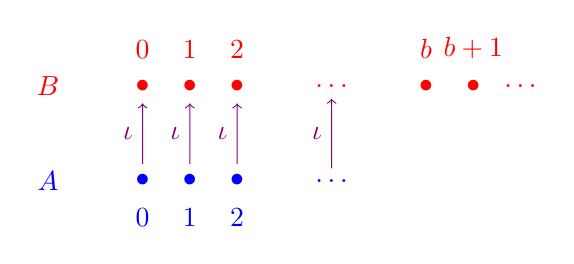
\begin{tikzpicture}[very thick, scale=0.6]
\begin{scope}[color=blue]
\node (A) at (0,0) {$A$};
\node(A0) at (2,0)[label=below:$0$]{$\bullet$};
\node(A1) at (3,0)[label=below:$1$]{$\bullet$};
\node(A2) at (4,0)[label=below:$2$]{$\bullet$};
\node (Adots) at (6,0) {$\ldots$};
\end{scope}
\begin{scope}[color=red]
\node (B) at (0,2) {$B$};
\node(B0) at (2,2)[label=above:$0$]{$\bullet$};
\node(B1) at (3,2)[label=above:$1$]{$\bullet$};
\node(B2) at (4,2)[label=above:$2$]{$\bullet$};
\node (Bdots) at (6,2) {$\ldots$};
\node (b) at (8,2) [label=above:$b$]{$\bullet$};
\node (bsucc) at (9,2) [label=above:$b+1$]{$\bullet$};
\node (Bdots2) at (10,2) {$\ldots$};
\end{scope}
\begin{scope}[color=red!50!blue]
\draw [->,thin] (A0) -- node [auto] {$\iota$} (B0);
\draw [->,thin] (A1) -- node [auto] {$\iota$} (B1);
\draw [->,thin] (A2) -- node [auto] {$\iota$} (B2);
\draw [->,thin] (Adots) -- node [auto] {$\iota$} (Bdots);
\end{scope}
\end{tikzpicture}
   \caption{\textcolor{blue}{$A$} is a sub-segment  of \textcolor{red}{$B$}}
   \label{fig:subsegment}
 \end{figure}




\index{Coq!Commands!Program}

We are now able to build an instance of \texttt{SubON}. 

\begin{Coqsrc}
Section Inclusion_ij.

  Variables i j : nat.
  Hypothesis Hij : (i < j)%nat.

   Remark Ltb_ij : Nat.ltb i j.
   Program Definition iota_ij  (alpha: t i) : t j :=  alpha.
 
   Let b : t j := exist _ i Ltb_ij.
   
   Global Instance F_incl_ij  : SubON  (FinOrd i) (FinOrd j) b iota_ij.
  (* ... *)

  End Inclusion_ij.

\end{Coqsrc}
         



\begin{remark}
 There is no interesting arihmetic on finite ordinals, since functions like successor, addition, etc.,  cannot be represented in \coq{} as \emph{total} functions.
\end{remark}

\paragraph{Related work}
Finite ordinals are also formalized in MathComp~\cite{SSR}.  See also Adam Chlipala's \emph{CPDT}~\cite{chlipalacpdt2011} for a thorough study of the use of dependent types.


\section{Isomorphism of ordinal notations}


In some cases we want to show that two notation systems describe the same segment (for instance $[0,3+\omega)$ and $[0,\omega($). For this purpose, one may prove that the two notation systems are order-isomorphic.

\index{Coq!Type classes}
\label{types:ON-iso} 
\begin{Coqsrc}
Class  ON_Iso 
       `(OA : @ON A ltA compareA)
       `(OB : @ON B ltB  compareB)
       (f : A -> B)
       (g : B -> A):=
  {
  iso_compare: forall x y : A, 
      compareB (f x) (f y) = compareA x y;
  iso_inv1 : forall a, g (f a)= a;
  iso_inv2 : forall b, f (g b) = b}.
\end{Coqsrc}

\index{Exercises}

\begin{exercise}
Let $i$ be some natural number. Prove that the notation systems 
\texttt{Omega} and \texttt{ON\_plus (OrdFin $i$) Omega} are isomorphic.

{\it \textbf{Note:s} This property reflects the equality $i+\omega=\omega$ we will prove in larger notation systems, as well as in Schütte's model}

This exercise is partially solved for $i=3$ (in ~\href{../src/html/hydras.OrdinalNotations.Example_3PlusOmega.html}{OrdinalNotations.Example\_3PlusOmega}).

\end{exercise}

\index{Projects}
\label{exo:ON-mult}
\begin{project}
Define in \coq{} the product of two ordinal notations $N_A$ and $N_B$.
If $A$ [resp. $B$] is the underlying type of $N_A$ [resp. $N_B$], the
product \texttt{ON\_mult $N_A$ $N_B$} is implemented over the cartesian product $B\times A$ (with the lexicographic ordering).

For instance, the
elements of the product \texttt{ON\_mult Omega (FinOrd 3)} are ordered as follows.
\[(0,0),(0,1),(0,2),(0,3),(0,4),\dots,{\color{red}(1,0),} (1,1),(1,2),\dots, {\color{red}(2,0)},(2,1),(2,2),\dots\]

Note that the elements of  \texttt{ON\_mult (FinOrd 3) Omega} are differently ordered (without limit ordinals):
\[(0,0),(1,0),(2,0),(0,1),(1,1),(2,1),(0,2),(1,2),(2,2),(0,3),\dots\]
(no limit ordinals).

Prove that \texttt{ON\_mult (FinOrd $i$) Omega} is isomorphic to
\texttt{Omega}  whilst
\texttt{Omega}  is a sub-notation of \texttt{ON\_mult Omega (FinOrd $i$)},
for any strictly positive $i$.
\end{project}

\index{Projects}
\begin{project}
\label{project:succ-limit-dec}
Add to the class \texttt{ON} the requirement that for any $\alpha$ it is decidable whether $\alpha$ is $0$, a successor or a limit ordinal.
\end{project}

\index{Projects}
\begin{project}
\label{project:on-setoid}
Reconsider the  class \texttt{ON}, with an equivalence instead of Leibniz equality.
\end{project}


%%%% ICI ICI

\section{Other ordinal notations}

\index{Projects}

\begin{project}
The directory \texttt{src/OmegaOmega} contains an ad-hoc formalization of $\omega^\omega$, contributed by Pascal Manoury. Every ordinal $\alpha$ is represented by a list $l$ whose elements are the coefficients of $\omega$ in  the Cantor normal form of $\alpha$ (in reverse order). For instance, the ordinal 
$\omega^{8}\times 5 + \omega^{6}\times 8 + \omega^2\times 10 + \omega + 7$ is represented by the list \texttt{[5;0;8;0;0.0;10,1,7]}. 


 Develop this representation and compare it with the other ordinal notations.



\end{project}

\index{Projects}

\begin{project}
Let $N_A$ be a notation system for ordinals strictly less than $\alpha$, 
with the strict order $(A,<_A)$. Please build the notation system
\texttt{ON\_Expl $N_A$}, on the type of multisets of elements of $A$
(or, if preferred, the type of non-increasing finite sequences on $A$,
provided with the lexicographic ordering on lists).

For instance, let us take $N_A=\texttt{Omega}$, and take $\alpha=\langle 4,4,2,1,0\rangle$,
 $\beta=\langle 4,3,3,3,3,3,2\rangle$, and $\gamma=\langle 5\rangle$. Then $\beta<\alpha<\gamma$. 

In contrast the list $\langle5,6,3,3\rangle$ is not non-increasing (\emph{i.e.} sorted w.r.t. $\geq$), so it is not to be considered.

Note that if the notation $N_A$ implements the ordinal 
$\alpha$,  the new notation $\omega^{N_A}$ must implement the ordinal $\varphi_0(\alpha)$, a.k.a. $\omega^\alpha$ (see chapter~\ref{chap:schutte})

\end{project}



\begin{remark}
 The set of ordinal terms in Cantor normal form (see Chap.~\ref{chap:T1}) and 
in Veblen normal form (see 
\href{../src/html/hydras.Gamma0.Gamma0.html}{Gamma0.Gamma0}) are shown to be ordinal notation systems, but there is a lot of work to be done in order to unify ad-hoc  definitions and proofs which were written before the definition of the \texttt{ON} type class.
\end{remark}







